\documentclass[1p]{elsarticle_modified}
%\bibliographystyle{elsarticle-num}

%\usepackage[colorlinks]{hyperref}
%\usepackage{abbrmath_seonhwa} %\Abb, \Ascr, \Acal ,\Abf, \Afrak
\usepackage{amsfonts}
\usepackage{amssymb}
\usepackage{amsmath}
\usepackage{amsthm}
\usepackage{scalefnt}
\usepackage{amsbsy}
\usepackage{kotex}
\usepackage{caption}
\usepackage{subfig}
\usepackage{color}
\usepackage{graphicx}
\usepackage{xcolor} %% white, black, red, green, blue, cyan, magenta, yellow
\usepackage{float}
\usepackage{setspace}
\usepackage{hyperref}

\usepackage{tikz}
\usetikzlibrary{arrows}

\usepackage{multirow}
\usepackage{array} % fixed length table
\usepackage{hhline}

%%%%%%%%%%%%%%%%%%%%%
\makeatletter
\renewcommand*\env@matrix[1][\arraystretch]{%
	\edef\arraystretch{#1}%
	\hskip -\arraycolsep
	\let\@ifnextchar\new@ifnextchar
	\array{*\c@MaxMatrixCols c}}
\makeatother %https://tex.stackexchange.com/questions/14071/how-can-i-increase-the-line-spacing-in-a-matrix
%%%%%%%%%%%%%%%

\usepackage[normalem]{ulem}

\newcommand{\msout}[1]{\ifmmode\text{\sout{\ensuremath{#1}}}\else\sout{#1}\fi}
%SOURCE: \msout is \stkout macro in https://tex.stackexchange.com/questions/20609/strikeout-in-math-mode

\newcommand{\cancel}[1]{
	\ifmmode
	{\color{red}\msout{#1}}
	\else
	{\color{red}\sout{#1}}
	\fi
}

\newcommand{\add}[1]{
	{\color{blue}\uwave{#1}}
}

\newcommand{\replace}[2]{
	\ifmmode
	{\color{red}\msout{#1}}{\color{blue}\uwave{#2}}
	\else
	{\color{red}\sout{#1}}{\color{blue}\uwave{#2}}
	\fi
}

\newcommand{\Sol}{\mathcal{S}} %segment
\newcommand{\D}{D} %diagram
\newcommand{\A}{\mathcal{A}} %arc


%%%%%%%%%%%%%%%%%%%%%%%%%%%%%5 test

\def\sl{\operatorname{\textup{SL}}(2,\Cbb)}
\def\psl{\operatorname{\textup{PSL}}(2,\Cbb)}
\def\quan{\mkern 1mu \triangleright \mkern 1mu}

\theoremstyle{definition}
\newtheorem{thm}{Theorem}[section]
\newtheorem{prop}[thm]{Proposition}
\newtheorem{lem}[thm]{Lemma}
\newtheorem{ques}[thm]{Question}
\newtheorem{cor}[thm]{Corollary}
\newtheorem{defn}[thm]{Definition}
\newtheorem{exam}[thm]{Example}
\newtheorem{rmk}[thm]{Remark}
\newtheorem{alg}[thm]{Algorithm}

\newcommand{\I}{\sqrt{-1}}
\begin{document}

%\begin{frontmatter}
%
%\title{Boundary parabolic representations of knots up to 8 crossings}
%
%%% Group authors per affiliation:
%\author{Yunhi Cho} 
%\address{Department of Mathematics, University of Seoul, Seoul, Korea}
%\ead{yhcho@uos.ac.kr}
%
%
%\author{Seonhwa Kim} %\fnref{s_kim}}
%\address{Center for Geometry and Physics, Institute for Basic Science, Pohang, 37673, Korea}
%\ead{ryeona17@ibs.re.kr}
%
%\author{Hyuk Kim}
%\address{Department of Mathematical Sciences, Seoul National University, Seoul 08826, Korea}
%\ead{hyukkim@snu.ac.kr}
%
%\author{Seokbeom Yoon}
%\address{Department of Mathematical Sciences, Seoul National University, Seoul, 08826,  Korea}
%\ead{sbyoon15@snu.ac.kr}
%
%\begin{abstract}
%We find all boundary parabolic representation of knots up to 8 crossings.
%
%\end{abstract}
%\begin{keyword}
%    \MSC[2010] 57M25 
%\end{keyword}
%
%\end{frontmatter}

%\linenumbers
%\tableofcontents
%
\newcommand\colored[1]{\textcolor{white}{\rule[-0.35ex]{0.8em}{1.4ex}}\kern-0.8em\color{red} #1}%
%\newcommand\colored[1]{\textcolor{white}{ #1}\kern-2.17ex	\textcolor{white}{ #1}\kern-1.81ex	\textcolor{white}{ #1}\kern-2.15ex\color{red}#1	}

{\Large $\underline{11n_{183}~(K11n_{183})}$}

\setlength{\tabcolsep}{10pt}
\renewcommand{\arraystretch}{1.6}
\vspace{1cm}\begin{tabular}{m{100pt}>{\centering\arraybackslash}m{274pt}}
\multirow{5}{120pt}{
	\centering
	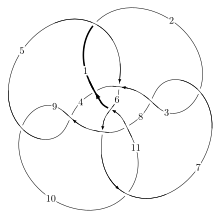
\includegraphics[width=112pt]{../../../GIT/diagram.site/Diagrams/png/799_11n_183.png}\\
\ \ \ A knot diagram\footnotemark}&
\allowdisplaybreaks
\textbf{Linearized knot diagam} \\
\cline{2-2}
 &
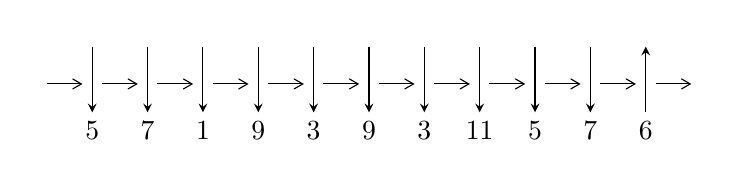
\begin{tikzpicture}[x=20pt, y=17pt]
	% nodes
	\node (C0) at (0, 0) {};
	\node (C1) at (1, 0) {};
	\node (C1U) at (1, +1) {};
	\node (C1D) at (1, -1) {5};

	\node (C2) at (2, 0) {};
	\node (C2U) at (2, +1) {};
	\node (C2D) at (2, -1) {7};

	\node (C3) at (3, 0) {};
	\node (C3U) at (3, +1) {};
	\node (C3D) at (3, -1) {1};

	\node (C4) at (4, 0) {};
	\node (C4U) at (4, +1) {};
	\node (C4D) at (4, -1) {9};

	\node (C5) at (5, 0) {};
	\node (C5U) at (5, +1) {};
	\node (C5D) at (5, -1) {3};

	\node (C6) at (6, 0) {};
	\node (C6U) at (6, +1) {};
	\node (C6D) at (6, -1) {9};

	\node (C7) at (7, 0) {};
	\node (C7U) at (7, +1) {};
	\node (C7D) at (7, -1) {3};

	\node (C8) at (8, 0) {};
	\node (C8U) at (8, +1) {};
	\node (C8D) at (8, -1) {11};

	\node (C9) at (9, 0) {};
	\node (C9U) at (9, +1) {};
	\node (C9D) at (9, -1) {5};

	\node (C10) at (10, 0) {};
	\node (C10U) at (10, +1) {};
	\node (C10D) at (10, -1) {7};

	\node (C11) at (11, 0) {};
	\node (C11U) at (11, +1) {};
	\node (C11D) at (11, -1) {6};
	\node (C12) at (12, 0) {};

	% arrows
	\draw[->,>={angle 60}]
	(C0) edge (C1) (C1) edge (C2) (C2) edge (C3) (C3) edge (C4) (C4) edge (C5) (C5) edge (C6) (C6) edge (C7) (C7) edge (C8) (C8) edge (C9) (C9) edge (C10) (C10) edge (C11) (C11) edge (C12) ;	\draw[->,>=stealth]
	(C1U) edge (C1D) (C2U) edge (C2D) (C3U) edge (C3D) (C4U) edge (C4D) (C5U) edge (C5D) (C6U) edge (C6D) (C7U) edge (C7D) (C8U) edge (C8D) (C9U) edge (C9D) (C10U) edge (C10D) (C11D) edge (C11U) ;
	\end{tikzpicture} \\
\hhline{~~} \\& 
\textbf{Solving Sequence} \\ \cline{2-2} 
 &
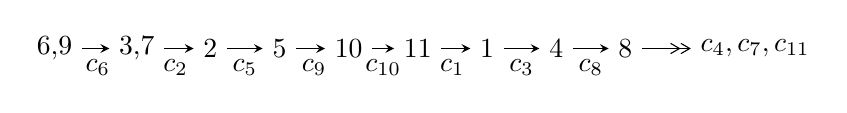
\begin{tikzpicture}[x=25pt, y=7pt]
	% node
	\node (A0) at (-1/8, 0) {6,9};
	\node (A1) at (17/16, 0) {3,7};
	\node (A2) at (17/8, 0) {2};
	\node (A3) at (25/8, 0) {5};
	\node (A4) at (33/8, 0) {10};
	\node (A5) at (41/8, 0) {11};
	\node (A6) at (49/8, 0) {1};
	\node (A7) at (57/8, 0) {4};
	\node (A8) at (65/8, 0) {8};
	\node (C1) at (1/2, -1) {$c_{6}$};
	\node (C2) at (13/8, -1) {$c_{2}$};
	\node (C3) at (21/8, -1) {$c_{5}$};
	\node (C4) at (29/8, -1) {$c_{9}$};
	\node (C5) at (37/8, -1) {$c_{10}$};
	\node (C6) at (45/8, -1) {$c_{1}$};
	\node (C7) at (53/8, -1) {$c_{3}$};
	\node (C8) at (61/8, -1) {$c_{8}$};
	\node (A9) at (10, 0) {$c_{4},c_{7},c_{11}$};

	% edge
	\draw[->,>=stealth]	
	(A0) edge (A1) (A1) edge (A2) (A2) edge (A3) (A3) edge (A4) (A4) edge (A5) (A5) edge (A6) (A6) edge (A7) (A7) edge (A8) ;
	\draw[->>,>={angle 60}]	
	(A8) edge (A9);
\end{tikzpicture} \\ 

\end{tabular} \\

\footnotetext{
The image of knot diagram is generated by the software ``\textbf{Draw programme}" developed by Andrew Bartholomew(\url{http://www.layer8.co.uk/maths/draw/index.htm\#Running-draw}), where we modified some parts for our purpose(\url{https://github.com/CATsTAILs/LinksPainter}).
}\phantom \\ \newline 
\centering \textbf{Ideals for irreducible components\footnotemark of $X_{\text{par}}$} 
 
\begin{align*}
I^u_{1}&=\langle 
b- u,\;5 u^6+6 u^5+13 u^4-7 u^3+29 u^2+9 a-11 u+16,\;u^7+u^6+2 u^5-3 u^4+5 u^3-3 u^2+4 u-1\rangle \\
I^u_{2}&=\langle 
b- u,\;54 u^5-72 u^4-84 u^3-80 u^2+11 a-85 u-184,\;u^6- u^5-2 u^4-2 u^3-2 u^2-4 u-1\rangle \\
I^u_{3}&=\langle 
37 u^7-61 u^6+51 u^5-60 u^4+86 u^3-191 u^2+29 b+214 u-54,\\
\phantom{I^u_{3}}&\phantom{= \langle  }-41 u^7+77 u^6-62 u^5+61 u^4-100 u^3+214 u^2+29 a-292 u+81,\\
\phantom{I^u_{3}}&\phantom{= \langle  }u^8-2 u^7+2 u^6-2 u^5+3 u^4-6 u^3+8 u^2-4 u+1\rangle \\
I^u_{4}&=\langle 
u^3+3 u^2+3 b+6 u+7,\;-2 u^3-21 u^2+39 a-57 u-59,\;u^4+4 u^3+9 u^2+10 u+13\rangle \\
I^u_{5}&=\langle 
b- u-1,\;a- u-1,\;u^2+u+1\rangle \\
I^u_{6}&=\langle 
b+u,\;a+4 u-9,\;u^2-2 u-1\rangle \\
I^u_{7}&=\langle 
b+u-1,\;3 a-2 u+2,\;u^2- u+3\rangle \\
I^u_{8}&=\langle 
b+u+1,\;a,\;u^2+u+1\rangle \\
I^u_{9}&=\langle 
b+1,\;a+1,\;u-1\rangle \\
I^u_{10}&=\langle 
b+u-1,\;a- u+1,\;u^2- u+1\rangle \\
\\
\end{align*}
\raggedright * 10 irreducible components of $\dim_{\mathbb{C}}=0$, with total 36 representations.\\
\footnotetext{All coefficients of polynomials are rational numbers. But the coefficients are sometimes approximated in decimal forms when there is not enough margin.}
\newpage
\renewcommand{\arraystretch}{1}
\centering \section*{I. $I^u_{1}= \langle b- u,\;5 u^6+6 u^5+\cdots+9 a+16,\;u^7+u^6+2 u^5-3 u^4+5 u^3-3 u^2+4 u-1 \rangle$}
\flushleft \textbf{(i) Arc colorings}\\
\begin{tabular}{m{7pt} m{180pt} m{7pt} m{180pt} }
\flushright $a_{6}=$&$\begin{pmatrix}1\\0\end{pmatrix}$ \\
\flushright $a_{9}=$&$\begin{pmatrix}0\\u\end{pmatrix}$ \\
\flushright $a_{3}=$&$\begin{pmatrix}-\frac{5}{9} u^6-\frac{2}{3} u^5+\cdots+\frac{11}{9} u-\frac{16}{9}\\u\end{pmatrix}$ \\
\flushright $a_{7}=$&$\begin{pmatrix}1\\u^2\end{pmatrix}$ \\
\flushright $a_{2}=$&$\begin{pmatrix}-\frac{1}{3} u^6-\frac{2}{3} u^4+\cdots+\frac{7}{3} u-\frac{5}{3}\\-\frac{1}{9} u^6-\frac{1}{3} u^5+\cdots-\frac{5}{9} u+\frac{4}{9}\end{pmatrix}$ \\
\flushright $a_{5}=$&$\begin{pmatrix}\frac{1}{9} u^6+\frac{1}{3} u^5+\cdots-\frac{4}{9} u+\frac{14}{9}\\- u^2\end{pmatrix}$ \\
\flushright $a_{10}=$&$\begin{pmatrix}-\frac{2}{9} u^6-\frac{2}{3} u^5+\cdots-\frac{19}{9} u-\frac{1}{9}\\-\frac{1}{9} u^6-\frac{1}{3} u^5+\cdots-\frac{5}{9} u+\frac{4}{9}\end{pmatrix}$ \\
\flushright $a_{11}=$&$\begin{pmatrix}-1\\-\frac{2}{9} u^6-\frac{2}{3} u^5+\cdots-\frac{19}{9} u+\frac{8}{9}\end{pmatrix}$ \\
\flushright $a_{1}=$&$\begin{pmatrix}-\frac{2}{9} u^6-\frac{2}{3} u^5+\cdots-\frac{19}{9} u-\frac{1}{9}\\-\frac{2}{9} u^6-\frac{2}{3} u^5+\cdots-\frac{19}{9} u+\frac{8}{9}\end{pmatrix}$ \\
\flushright $a_{4}=$&$\begin{pmatrix}-\frac{1}{9} u^6-\frac{1}{3} u^5+\cdots+\frac{4}{9} u-\frac{14}{9}\\\frac{4}{9} u^6+\frac{1}{3} u^5+\cdots-\frac{7}{9} u+\frac{2}{9}\end{pmatrix}$ \\
\flushright $a_{8}=$&$\begin{pmatrix}u\\\frac{4}{9} u^6+\frac{1}{3} u^5+\cdots-\frac{7}{9} u+\frac{2}{9}\end{pmatrix}$\\ \flushright $a_{8}=$&$\begin{pmatrix}u\\\frac{4}{9} u^6+\frac{1}{3} u^5+\cdots-\frac{7}{9} u+\frac{2}{9}\end{pmatrix}$\\&\end{tabular}
\flushleft \textbf{(ii) Obstruction class $= -1$}\\~\\
\flushleft \textbf{(iii) Cusp Shapes $= -\frac{26}{9} u^6-\frac{8}{3} u^5-\frac{28}{9} u^4+\frac{112}{9} u^3-\frac{86}{9} u^2+\frac{14}{9} u-\frac{130}{9}$}\\~\\
\newpage\renewcommand{\arraystretch}{1}
\flushleft \textbf{(iv) u-Polynomials at the component}\newline \\
\begin{tabular}{m{50pt}|m{274pt}}
Crossings & \hspace{64pt}u-Polynomials at each crossing \\
\hline $$\begin{aligned}c_{1},c_{10}\end{aligned}$$&$\begin{aligned}
&u^7+4 u^6+24 u^5+58 u^4+139 u^3+194 u^2+120 u+24
\end{aligned}$\\
\hline $$\begin{aligned}c_{2},c_{4},c_{7}\\c_{9}\end{aligned}$$&$\begin{aligned}
&u^7+u^6+8 u^5- u^4+12 u^3-10 u^2-2 u+2
\end{aligned}$\\
\hline $$\begin{aligned}c_{3},c_{5},c_{6}\\c_{8}\end{aligned}$$&$\begin{aligned}
&u^7- u^6+2 u^5+3 u^4+5 u^3+3 u^2+4 u+1
\end{aligned}$\\
\hline $$\begin{aligned}c_{11}\end{aligned}$$&$\begin{aligned}
&u^7+7 u^6+28 u^5+69 u^4+106 u^3+96 u^2+48 u+8
\end{aligned}$\\
\hline
\end{tabular}\\~\\
\newpage\renewcommand{\arraystretch}{1}
\flushleft \textbf{(v) Riley Polynomials at the component}\newline \\
\begin{tabular}{m{50pt}|m{274pt}}
Crossings & \hspace{64pt}Riley Polynomials at each crossing \\
\hline $$\begin{aligned}c_{1},c_{10}\end{aligned}$$&$\begin{aligned}
&y^7+32 y^6+390 y^5+1996 y^4+2385 y^3-7060 y^2+5088 y-576
\end{aligned}$\\
\hline $$\begin{aligned}c_{2},c_{4},c_{7}\\c_{9}\end{aligned}$$&$\begin{aligned}
&y^7+15 y^6+90 y^5+207 y^4+88 y^3-144 y^2+44 y-4
\end{aligned}$\\
\hline $$\begin{aligned}c_{3},c_{5},c_{6}\\c_{8}\end{aligned}$$&$\begin{aligned}
&y^7+3 y^6+20 y^5+25 y^4+25 y^3+25 y^2+10 y-1
\end{aligned}$\\
\hline $$\begin{aligned}c_{11}\end{aligned}$$&$\begin{aligned}
&y^7+7 y^6+30 y^5-73 y^4+564 y^3-144 y^2+768 y-64
\end{aligned}$\\
\hline
\end{tabular}\\~\\
\newpage\flushleft \textbf{(vi) Complex Volumes and Cusp Shapes}
$$\begin{array}{c|c|c}  
\text{Solutions to }I^u_{1}& \I (\text{vol} + \sqrt{-1}CS) & \text{Cusp shape}\\
 \hline 
\begin{aligned}
u &= \phantom{-}0.757011 + 0.685123 I \\
a &= \phantom{-}0.681482 - 1.170220 I \\
b &= \phantom{-}0.757011 + 0.685123 I\end{aligned}
 & -1.68375 - 3.49152 I & -15.3039 + 5.7802 I \\ \hline\begin{aligned}
u &= \phantom{-}0.757011 - 0.685123 I \\
a &= \phantom{-}0.681482 + 1.170220 I \\
b &= \phantom{-}0.757011 - 0.685123 I\end{aligned}
 & -1.68375 + 3.49152 I & -15.3039 - 5.7802 I \\ \hline\begin{aligned}
u &= -0.134406 + 0.899226 I \\
a &= \phantom{-}0.516003 + 0.736811 I \\
b &= -0.134406 + 0.899226 I\end{aligned}
 & \phantom{-}10.56250 + 1.19923 I & -2.68829 - 5.87566 I \\ \hline\begin{aligned}
u &= -0.134406 - 0.899226 I \\
a &= \phantom{-}0.516003 - 0.736811 I \\
b &= -0.134406 - 0.899226 I\end{aligned}
 & \phantom{-}10.56250 - 1.19923 I & -2.68829 + 5.87566 I \\ \hline\begin{aligned}
u &= \phantom{-}0.285988\phantom{ +0.000000I} \\
a &= -1.68483\phantom{ +0.000000I} \\
b &= \phantom{-}0.285988\phantom{ +0.000000I}\end{aligned}
 & -0.666622\phantom{ +0.000000I} & -14.5180\phantom{ +0.000000I} \\ \hline\begin{aligned}
u &= -1.26560 + 1.56709 I \\
a &= -0.855070 - 0.684725 I \\
b &= -1.26560 + 1.56709 I\end{aligned}
 & \phantom{-}14.4836 + 11.4109 I & -7.74903 - 4.57488 I \\ \hline\begin{aligned}
u &= -1.26560 - 1.56709 I \\
a &= -0.855070 + 0.684725 I \\
b &= -1.26560 - 1.56709 I\end{aligned}
 & \phantom{-}14.4836 - 11.4109 I & -7.74903 + 4.57488 I\\
 \hline 
 \end{array}$$\newpage\newpage\renewcommand{\arraystretch}{1}
\centering \section*{II. $I^u_{2}= \langle b- u,\;54 u^5-72 u^4+\cdots+11 a-184,\;u^6- u^5-2 u^4-2 u^3-2 u^2-4 u-1 \rangle$}
\flushleft \textbf{(i) Arc colorings}\\
\begin{tabular}{m{7pt} m{180pt} m{7pt} m{180pt} }
\flushright $a_{6}=$&$\begin{pmatrix}1\\0\end{pmatrix}$ \\
\flushright $a_{9}=$&$\begin{pmatrix}0\\u\end{pmatrix}$ \\
\flushright $a_{3}=$&$\begin{pmatrix}-4.90909 u^{5}+6.54545 u^{4}+\cdots+7.72727 u+16.7273\\u\end{pmatrix}$ \\
\flushright $a_{7}=$&$\begin{pmatrix}1\\u^2\end{pmatrix}$ \\
\flushright $a_{2}=$&$\begin{pmatrix}-4.36364 u^{5}+5.81818 u^{4}+\cdots+7.09091 u+15.0909\\-0.272727 u^{5}+0.363636 u^{4}+\cdots+0.818182 u-0.181818\end{pmatrix}$ \\
\flushright $a_{5}=$&$\begin{pmatrix}-1.63636 u^{5}+2.18182 u^{4}+\cdots+2.90909 u+5.90909\\- u^2\end{pmatrix}$ \\
\flushright $a_{10}=$&$\begin{pmatrix}-2.45455 u^{5}+3.27273 u^{4}+\cdots+3.36364 u+8.36364\\-0.272727 u^{5}+0.363636 u^{4}+\cdots+0.818182 u-0.181818\end{pmatrix}$ \\
\flushright $a_{11}=$&$\begin{pmatrix}-2.45455 u^{5}+3.27273 u^{4}+\cdots+3.36364 u+9.36364\\-0.272727 u^{5}+0.363636 u^{4}+\cdots+0.818182 u-0.181818\end{pmatrix}$ \\
\flushright $a_{1}=$&$\begin{pmatrix}-2.72727 u^{5}+3.63636 u^{4}+\cdots+4.18182 u+9.18182\\-0.272727 u^{5}+0.363636 u^{4}+\cdots+0.818182 u-0.181818\end{pmatrix}$ \\
\flushright $a_{4}=$&$\begin{pmatrix}1.63636 u^{5}-2.18182 u^{4}+\cdots-2.90909 u-5.90909\\-0.181818 u^{5}-0.0909091 u^{4}+\cdots+0.545455 u+0.545455\end{pmatrix}$ \\
\flushright $a_{8}=$&$\begin{pmatrix}6.72727 u^{5}-8.63636 u^{4}+\cdots-10.1818 u-23.1818\\-0.181818 u^{5}-0.0909091 u^{4}+\cdots+0.545455 u+0.545455\end{pmatrix}$\\ \flushright $a_{8}=$&$\begin{pmatrix}6.72727 u^{5}-8.63636 u^{4}+\cdots-10.1818 u-23.1818\\-0.181818 u^{5}-0.0909091 u^{4}+\cdots+0.545455 u+0.545455\end{pmatrix}$\\&\end{tabular}
\flushleft \textbf{(ii) Obstruction class $= -1$}\\~\\
\flushleft \textbf{(iii) Cusp Shapes $= -\frac{84}{11} u^5+\frac{112}{11} u^4+\frac{116}{11} u^3+\frac{188}{11} u^2+\frac{164}{11} u+\frac{274}{11}$}\\~\\
\newpage\renewcommand{\arraystretch}{1}
\flushleft \textbf{(iv) u-Polynomials at the component}\newline \\
\begin{tabular}{m{50pt}|m{274pt}}
Crossings & \hspace{64pt}u-Polynomials at each crossing \\
\hline $$\begin{aligned}c_{1},c_{10}\end{aligned}$$&$\begin{aligned}
&(u-1)^6
\end{aligned}$\\
\hline $$\begin{aligned}c_{2},c_{4},c_{7}\\c_{9}\end{aligned}$$&$\begin{aligned}
&(u^3- u^2-1)^2
\end{aligned}$\\
\hline $$\begin{aligned}c_{3},c_{5},c_{6}\\c_{8}\end{aligned}$$&$\begin{aligned}
&u^6+u^5-2 u^4+2 u^3-2 u^2+4 u-1
\end{aligned}$\\
\hline $$\begin{aligned}c_{11}\end{aligned}$$&$\begin{aligned}
&(u^3-3 u^2+4 u-1)^2
\end{aligned}$\\
\hline
\end{tabular}\\~\\
\newpage\renewcommand{\arraystretch}{1}
\flushleft \textbf{(v) Riley Polynomials at the component}\newline \\
\begin{tabular}{m{50pt}|m{274pt}}
Crossings & \hspace{64pt}Riley Polynomials at each crossing \\
\hline $$\begin{aligned}c_{1},c_{10}\end{aligned}$$&$\begin{aligned}
&(y-1)^6
\end{aligned}$\\
\hline $$\begin{aligned}c_{2},c_{4},c_{7}\\c_{9}\end{aligned}$$&$\begin{aligned}
&(y^3- y^2-2 y-1)^2
\end{aligned}$\\
\hline $$\begin{aligned}c_{3},c_{5},c_{6}\\c_{8}\end{aligned}$$&$\begin{aligned}
&y^6-5 y^5-4 y^4-6 y^3-8 y^2-12 y+1
\end{aligned}$\\
\hline $$\begin{aligned}c_{11}\end{aligned}$$&$\begin{aligned}
&(y^3- y^2+10 y-1)^2
\end{aligned}$\\
\hline
\end{tabular}\\~\\
\newpage\flushleft \textbf{(vi) Complex Volumes and Cusp Shapes}
$$\begin{array}{c|c|c}  
\text{Solutions to }I^u_{2}& \I (\text{vol} + \sqrt{-1}CS) & \text{Cusp shape}\\
 \hline 
\begin{aligned}
u &= \phantom{-}0.346535 + 1.017670 I \\
a &= \phantom{-}0.040902 - 0.214369 I \\
b &= \phantom{-}0.346535 + 1.017670 I\end{aligned}
 & \phantom{-}1.59057 - 4.74950 I & -3.95625 + 7.59808 I \\ \hline\begin{aligned}
u &= \phantom{-}0.346535 - 1.017670 I \\
a &= \phantom{-}0.040902 + 0.214369 I \\
b &= \phantom{-}0.346535 - 1.017670 I\end{aligned}
 & \phantom{-}1.59057 + 4.74950 I & -3.95625 - 7.59808 I \\ \hline\begin{aligned}
u &= -0.920485 + 0.648681 I \\
a &= -1.37622 - 0.47421 I \\
b &= -0.920485 + 0.648681 I\end{aligned}
 & \phantom{-}1.59057 + 4.74950 I & -3.95625 - 7.59808 I \\ \hline\begin{aligned}
u &= -0.920485 - 0.648681 I \\
a &= -1.37622 + 0.47421 I \\
b &= -0.920485 - 0.648681 I\end{aligned}
 & \phantom{-}1.59057 - 4.74950 I & -3.95625 + 7.59808 I \\ \hline\begin{aligned}
u &= -0.280929\phantom{ +0.000000I} \\
a &= \phantom{-}15.0105\phantom{ +0.000000I} \\
b &= -0.280929\phantom{ +0.000000I}\end{aligned}
 & -8.11594\phantom{ +0.000000I} & \phantom{-}21.9130\phantom{ +0.000000I} \\ \hline\begin{aligned}
u &= \phantom{-}2.42883\phantom{ +0.000000I} \\
a &= \phantom{-}0.660157\phantom{ +0.000000I} \\
b &= \phantom{-}2.42883\phantom{ +0.000000I}\end{aligned}
 & -8.11594\phantom{ +0.000000I} & \phantom{-}21.9130\phantom{ +0.000000I}\\
 \hline 
 \end{array}$$\newpage\newpage\renewcommand{\arraystretch}{1}
\centering \section*{III. $I^u_{3}= \langle 37 u^7-61 u^6+\cdots+29 b-54,\;-41 u^7+77 u^6+\cdots+29 a+81,\;u^8-2 u^7+\cdots-4 u+1 \rangle$}
\flushleft \textbf{(i) Arc colorings}\\
\begin{tabular}{m{7pt} m{180pt} m{7pt} m{180pt} }
\flushright $a_{6}=$&$\begin{pmatrix}1\\0\end{pmatrix}$ \\
\flushright $a_{9}=$&$\begin{pmatrix}0\\u\end{pmatrix}$ \\
\flushright $a_{3}=$&$\begin{pmatrix}1.41379 u^{7}-2.65517 u^{6}+\cdots+10.0690 u-2.79310\\-1.27586 u^{7}+2.10345 u^{6}+\cdots-7.37931 u+1.86207\end{pmatrix}$ \\
\flushright $a_{7}=$&$\begin{pmatrix}1\\u^2\end{pmatrix}$ \\
\flushright $a_{2}=$&$\begin{pmatrix}0.482759 u^{7}-0.931034 u^{6}+\cdots+3.41379 u-0.758621\\- u^7+2 u^6-2 u^5+2 u^4-3 u^3+6 u^2-7 u+2\end{pmatrix}$ \\
\flushright $a_{5}=$&$\begin{pmatrix}0.655172 u^{7}-1.62069 u^{6}+\cdots+6.27586 u-3.17241\\-0.551724 u^{7}+1.20690 u^{6}+\cdots-4.75862 u+2.72414\end{pmatrix}$ \\
\flushright $a_{10}=$&$\begin{pmatrix}0.310345 u^{7}-1.24138 u^{6}+\cdots+4.55172 u-2.34483\\-0.827586 u^{7}+1.31034 u^{6}+\cdots-4.13793 u+2.58621\end{pmatrix}$ \\
\flushright $a_{11}=$&$\begin{pmatrix}0.379310 u^{7}-1.51724 u^{6}+\cdots+5.89655 u-4.31034\\-0.551724 u^{7}+1.20690 u^{6}+\cdots-4.75862 u+2.72414\end{pmatrix}$ \\
\flushright $a_{1}=$&$\begin{pmatrix}-0.172414 u^{7}-0.310345 u^{6}+\cdots+1.13793 u-1.58621\\-0.551724 u^{7}+1.20690 u^{6}+\cdots-4.75862 u+2.72414\end{pmatrix}$ \\
\flushright $a_{4}=$&$\begin{pmatrix}0.655172 u^{7}-1.62069 u^{6}+\cdots+6.27586 u-3.17241\\-0.172414 u^{7}+0.689655 u^{6}+\cdots-2.86207 u+2.41379\end{pmatrix}$ \\
\flushright $a_{8}=$&$\begin{pmatrix}0.448276 u^{7}+0.206897 u^{6}+\cdots-0.758621 u+3.72414\\0.172414 u^{7}-0.689655 u^{6}+\cdots+2.86207 u-2.41379\end{pmatrix}$\\ \flushright $a_{8}=$&$\begin{pmatrix}0.448276 u^{7}+0.206897 u^{6}+\cdots-0.758621 u+3.72414\\0.172414 u^{7}-0.689655 u^{6}+\cdots+2.86207 u-2.41379\end{pmatrix}$\\&\end{tabular}
\flushleft \textbf{(ii) Obstruction class $= 1$}\\~\\
\flushleft \textbf{(iii) Cusp Shapes $= \frac{48}{29} u^7-\frac{76}{29} u^6+\frac{74}{29} u^5-\frac{70}{29} u^4+\frac{110}{29} u^3-\frac{218}{29} u^2+\frac{298}{29} u-\frac{324}{29}$}\\~\\
\newpage\renewcommand{\arraystretch}{1}
\flushleft \textbf{(iv) u-Polynomials at the component}\newline \\
\begin{tabular}{m{50pt}|m{274pt}}
Crossings & \hspace{64pt}u-Polynomials at each crossing \\
\hline $$\begin{aligned}c_{1}\end{aligned}$$&$\begin{aligned}
&(u^4-2 u^3+2)^2
\end{aligned}$\\
\hline $$\begin{aligned}c_{2},c_{4},c_{7}\\c_{9}\end{aligned}$$&$\begin{aligned}
&(u^4+u^2-1)^2
\end{aligned}$\\
\hline $$\begin{aligned}c_{3},c_{5}\end{aligned}$$&$\begin{aligned}
&u^8+2 u^7+2 u^6+2 u^5+3 u^4+6 u^3+8 u^2+4 u+1
\end{aligned}$\\
\hline $$\begin{aligned}c_{6},c_{8}\end{aligned}$$&$\begin{aligned}
&u^8-2 u^7+2 u^6-2 u^5+3 u^4-6 u^3+8 u^2-4 u+1
\end{aligned}$\\
\hline $$\begin{aligned}c_{10}\end{aligned}$$&$\begin{aligned}
&(u^4+2 u^3+2)^2
\end{aligned}$\\
\hline $$\begin{aligned}c_{11}\end{aligned}$$&$\begin{aligned}
&(u^4-2 u^2+5)^2
\end{aligned}$\\
\hline
\end{tabular}\\~\\
\newpage\renewcommand{\arraystretch}{1}
\flushleft \textbf{(v) Riley Polynomials at the component}\newline \\
\begin{tabular}{m{50pt}|m{274pt}}
Crossings & \hspace{64pt}Riley Polynomials at each crossing \\
\hline $$\begin{aligned}c_{1},c_{10}\end{aligned}$$&$\begin{aligned}
&(y^4-4 y^3+4 y^2+4)^2
\end{aligned}$\\
\hline $$\begin{aligned}c_{2},c_{4},c_{7}\\c_{9}\end{aligned}$$&$\begin{aligned}
&(y^2+y-1)^4
\end{aligned}$\\
\hline $$\begin{aligned}c_{3},c_{5},c_{6}\\c_{8}\end{aligned}$$&$\begin{aligned}
&y^8+2 y^6+3 y^4+22 y^2+1
\end{aligned}$\\
\hline $$\begin{aligned}c_{11}\end{aligned}$$&$\begin{aligned}
&(y^2-2 y+5)^4
\end{aligned}$\\
\hline
\end{tabular}\\~\\
\newpage\flushleft \textbf{(vi) Complex Volumes and Cusp Shapes}
$$\begin{array}{c|c|c}  
\text{Solutions to }I^u_{3}& \I (\text{vol} + \sqrt{-1}CS) & \text{Cusp shape}\\
 \hline 
\begin{aligned}
u &= \phantom{-}0.415941 + 1.202090 I \\
a &= \phantom{-}0.415941 + 0.584059 I \\
b &= -0.326993 - 0.326993 I\end{aligned}
 & \phantom{-}0.82247 - 3.66386 I & -8.00000 + 2.00000 I \\ \hline\begin{aligned}
u &= \phantom{-}0.415941 - 1.202090 I \\
a &= \phantom{-}0.415941 - 0.584059 I \\
b &= -0.326993 + 0.326993 I\end{aligned}
 & \phantom{-}0.82247 + 3.66386 I & -8.00000 - 2.00000 I \\ \hline\begin{aligned}
u &= \phantom{-}1.202090 + 0.415941 I \\
a &= \phantom{-}1.202090 - 0.202093 I \\
b &= \phantom{-}0.945027 + 0.945027 I\end{aligned}
 & \phantom{-}0.82247 - 3.66386 I & -8.00000 + 2.00000 I \\ \hline\begin{aligned}
u &= \phantom{-}1.202090 - 0.415941 I \\
a &= \phantom{-}1.202090 + 0.202093 I \\
b &= \phantom{-}0.945027 - 0.945027 I\end{aligned}
 & \phantom{-}0.82247 + 3.66386 I & -8.00000 - 2.00000 I \\ \hline\begin{aligned}
u &= -0.945027 + 0.945027 I \\
a &= -0.945027 - 0.673007 I \\
b &= -1.202090 + 0.415941 I\end{aligned}
 & \phantom{-}0.82247 + 3.66386 I & -8.00000 - 2.00000 I \\ \hline\begin{aligned}
u &= -0.945027 - 0.945027 I \\
a &= -0.945027 + 0.673007 I \\
b &= -1.202090 - 0.415941 I\end{aligned}
 & \phantom{-}0.82247 - 3.66386 I & -8.00000 + 2.00000 I \\ \hline\begin{aligned}
u &= \phantom{-}0.326993 + 0.326993 I \\
a &= \phantom{-}0.32699 + 1.94503 I \\
b &= -0.415941 - 1.202090 I\end{aligned}
 & \phantom{-}0.82247 - 3.66386 I & -8.00000 + 2.00000 I \\ \hline\begin{aligned}
u &= \phantom{-}0.326993 - 0.326993 I \\
a &= \phantom{-}0.32699 - 1.94503 I \\
b &= -0.415941 + 1.202090 I\end{aligned}
 & \phantom{-}0.82247 + 3.66386 I & -8.00000 - 2.00000 I\\
 \hline 
 \end{array}$$\newpage\newpage\renewcommand{\arraystretch}{1}
\centering \section*{IV. $I^u_{4}= \langle u^3+3 u^2+3 b+6 u+7,\;-2 u^3-21 u^2+39 a-57 u-59,\;u^4+4 u^3+9 u^2+10 u+13 \rangle$}
\flushleft \textbf{(i) Arc colorings}\\
\begin{tabular}{m{7pt} m{180pt} m{7pt} m{180pt} }
\flushright $a_{6}=$&$\begin{pmatrix}1\\0\end{pmatrix}$ \\
\flushright $a_{9}=$&$\begin{pmatrix}0\\u\end{pmatrix}$ \\
\flushright $a_{3}=$&$\begin{pmatrix}0.0512821 u^{3}+0.538462 u^{2}+1.46154 u+1.51282\\-\frac{1}{3} u^3- u^2-2 u-\frac{7}{3}\end{pmatrix}$ \\
\flushright $a_{7}=$&$\begin{pmatrix}1\\u^2\end{pmatrix}$ \\
\flushright $a_{2}=$&$\begin{pmatrix}0.0512821 u^{3}+1.53846 u^{2}+3.46154 u+3.51282\\-\frac{7}{3} u^3-8 u^2-12 u-\frac{46}{3}\end{pmatrix}$ \\
\flushright $a_{5}=$&$\begin{pmatrix}0.230769 u^{3}+0.923077 u^{2}+1.07692 u+0.307692\\-\frac{2}{3} u^3- u^2-2 u+\frac{1}{3}\end{pmatrix}$ \\
\flushright $a_{10}=$&$\begin{pmatrix}-0.307692 u^{3}-1.23077 u^{2}-3.76923 u-5.07692\\-\frac{4}{3} u^3-3 u^2+u-\frac{10}{3}\end{pmatrix}$ \\
\flushright $a_{11}=$&$\begin{pmatrix}0.0256410 u^{3}-0.230769 u^{2}-0.769231 u-1.74359\\1\end{pmatrix}$ \\
\flushright $a_{1}=$&$\begin{pmatrix}0.0256410 u^{3}-0.230769 u^{2}-0.769231 u-0.743590\\1\end{pmatrix}$ \\
\flushright $a_{4}=$&$\begin{pmatrix}-0.230769 u^{3}-0.923077 u^{2}-1.07692 u-0.307692\\-\frac{1}{3} u^3- u^2- u-\frac{1}{3}\end{pmatrix}$ \\
\flushright $a_{8}=$&$\begin{pmatrix}0.435897 u^{3}+1.07692 u^{2}+0.923077 u-1.64103\\-\frac{1}{3} u^3- u^2- u-\frac{1}{3}\end{pmatrix}$\\ \flushright $a_{8}=$&$\begin{pmatrix}0.435897 u^{3}+1.07692 u^{2}+0.923077 u-1.64103\\-\frac{1}{3} u^3- u^2- u-\frac{1}{3}\end{pmatrix}$\\&\end{tabular}
\flushleft \textbf{(ii) Obstruction class $= -1$}\\~\\
\flushleft \textbf{(iii) Cusp Shapes $= -6$}\\~\\
\newpage\renewcommand{\arraystretch}{1}
\flushleft \textbf{(iv) u-Polynomials at the component}\newline \\
\begin{tabular}{m{50pt}|m{274pt}}
Crossings & \hspace{64pt}u-Polynomials at each crossing \\
\hline $$\begin{aligned}c_{1},c_{10}\end{aligned}$$&$\begin{aligned}
&(u^2-2 u+10)^2
\end{aligned}$\\
\hline $$\begin{aligned}c_{2},c_{4},c_{7}\\c_{9}\end{aligned}$$&$\begin{aligned}
&(u^2- u+7)^2
\end{aligned}$\\
\hline $$\begin{aligned}c_{3},c_{5},c_{6}\\c_{8}\end{aligned}$$&$\begin{aligned}
&u^4-4 u^3+9 u^2-10 u+13
\end{aligned}$\\
\hline $$\begin{aligned}c_{11}\end{aligned}$$&$\begin{aligned}
&(u+1)^4
\end{aligned}$\\
\hline
\end{tabular}\\~\\
\newpage\renewcommand{\arraystretch}{1}
\flushleft \textbf{(v) Riley Polynomials at the component}\newline \\
\begin{tabular}{m{50pt}|m{274pt}}
Crossings & \hspace{64pt}Riley Polynomials at each crossing \\
\hline $$\begin{aligned}c_{1},c_{10}\end{aligned}$$&$\begin{aligned}
&(y^2+16 y+100)^2
\end{aligned}$\\
\hline $$\begin{aligned}c_{2},c_{4},c_{7}\\c_{9}\end{aligned}$$&$\begin{aligned}
&(y^2+13 y+49)^2
\end{aligned}$\\
\hline $$\begin{aligned}c_{3},c_{5},c_{6}\\c_{8}\end{aligned}$$&$\begin{aligned}
&y^4+2 y^3+27 y^2+134 y+169
\end{aligned}$\\
\hline $$\begin{aligned}c_{11}\end{aligned}$$&$\begin{aligned}
&(y-1)^4
\end{aligned}$\\
\hline
\end{tabular}\\~\\
\newpage\flushleft \textbf{(vi) Complex Volumes and Cusp Shapes}
$$\begin{array}{c|c|c}  
\text{Solutions to }I^u_{4}& \I (\text{vol} + \sqrt{-1}CS) & \text{Cusp shape}\\
 \hline 
\begin{aligned}
u &= -0.13397 + 1.50000 I \\
a &= \phantom{-}0.16139 + 1.80695 I \\
b &= -0.13397 - 1.50000 I\end{aligned}
 & \phantom{-}13.1595\phantom{ +0.000000I} & -6.00000\phantom{ +0.000000I} \\ \hline\begin{aligned}
u &= -0.13397 - 1.50000 I \\
a &= \phantom{-}0.16139 - 1.80695 I \\
b &= -0.13397 + 1.50000 I\end{aligned}
 & \phantom{-}13.1595\phantom{ +0.000000I} & -6.00000\phantom{ +0.000000I} \\ \hline\begin{aligned}
u &= -1.86603 + 1.50000 I \\
a &= -0.238314 - 0.191568 I \\
b &= -1.86603 - 1.50000 I\end{aligned}
 & \phantom{-}13.1595\phantom{ +0.000000I} & -6.00000\phantom{ +0.000000I} \\ \hline\begin{aligned}
u &= -1.86603 - 1.50000 I \\
a &= -0.238314 + 0.191568 I \\
b &= -1.86603 + 1.50000 I\end{aligned}
 & \phantom{-}13.1595\phantom{ +0.000000I} & -6.00000\phantom{ +0.000000I}\\
 \hline 
 \end{array}$$\newpage\newpage\renewcommand{\arraystretch}{1}
\centering \section*{V. $I^u_{5}= \langle b- u-1,\;a- u-1,\;u^2+u+1 \rangle$}
\flushleft \textbf{(i) Arc colorings}\\
\begin{tabular}{m{7pt} m{180pt} m{7pt} m{180pt} }
\flushright $a_{6}=$&$\begin{pmatrix}1\\0\end{pmatrix}$ \\
\flushright $a_{9}=$&$\begin{pmatrix}0\\u\end{pmatrix}$ \\
\flushright $a_{3}=$&$\begin{pmatrix}u+1\\u+1\end{pmatrix}$ \\
\flushright $a_{7}=$&$\begin{pmatrix}1\\- u-1\end{pmatrix}$ \\
\flushright $a_{2}=$&$\begin{pmatrix}3 u+2\\2\end{pmatrix}$ \\
\flushright $a_{5}=$&$\begin{pmatrix}- u+1\\- u\end{pmatrix}$ \\
\flushright $a_{10}=$&$\begin{pmatrix}-3 u-3\\-2\end{pmatrix}$ \\
\flushright $a_{11}=$&$\begin{pmatrix}-1\\-2 u-1\end{pmatrix}$ \\
\flushright $a_{1}=$&$\begin{pmatrix}-2 u-2\\-2 u-1\end{pmatrix}$ \\
\flushright $a_{4}=$&$\begin{pmatrix}- u+1\\2\end{pmatrix}$ \\
\flushright $a_{8}=$&$\begin{pmatrix}u\\-2\end{pmatrix}$\\ \flushright $a_{8}=$&$\begin{pmatrix}u\\-2\end{pmatrix}$\\&\end{tabular}
\flushleft \textbf{(ii) Obstruction class $= 1$}\\~\\
\flushleft \textbf{(iii) Cusp Shapes $= -9$}\\~\\
\newpage\renewcommand{\arraystretch}{1}
\flushleft \textbf{(iv) u-Polynomials at the component}\newline \\
\begin{tabular}{m{50pt}|m{274pt}}
Crossings & \hspace{64pt}u-Polynomials at each crossing \\
\hline $$\begin{aligned}c_{1}\end{aligned}$$&$\begin{aligned}
&u^2+u+7
\end{aligned}$\\
\hline $$\begin{aligned}c_{2},c_{4},c_{7}\\c_{9},c_{11}\end{aligned}$$&$\begin{aligned}
&u^2+3
\end{aligned}$\\
\hline $$\begin{aligned}c_{3},c_{5}\end{aligned}$$&$\begin{aligned}
&u^2- u+1
\end{aligned}$\\
\hline $$\begin{aligned}c_{6},c_{8}\end{aligned}$$&$\begin{aligned}
&u^2+u+1
\end{aligned}$\\
\hline $$\begin{aligned}c_{10}\end{aligned}$$&$\begin{aligned}
&u^2- u+7
\end{aligned}$\\
\hline
\end{tabular}\\~\\
\newpage\renewcommand{\arraystretch}{1}
\flushleft \textbf{(v) Riley Polynomials at the component}\newline \\
\begin{tabular}{m{50pt}|m{274pt}}
Crossings & \hspace{64pt}Riley Polynomials at each crossing \\
\hline $$\begin{aligned}c_{1},c_{10}\end{aligned}$$&$\begin{aligned}
&y^2+13 y+49
\end{aligned}$\\
\hline $$\begin{aligned}c_{2},c_{4},c_{7}\\c_{9},c_{11}\end{aligned}$$&$\begin{aligned}
&(y+3)^2
\end{aligned}$\\
\hline $$\begin{aligned}c_{3},c_{5},c_{6}\\c_{8}\end{aligned}$$&$\begin{aligned}
&y^2+y+1
\end{aligned}$\\
\hline
\end{tabular}\\~\\
\newpage\flushleft \textbf{(vi) Complex Volumes and Cusp Shapes}
$$\begin{array}{c|c|c}  
\text{Solutions to }I^u_{5}& \I (\text{vol} + \sqrt{-1}CS) & \text{Cusp shape}\\
 \hline 
\begin{aligned}
u &= -0.500000 + 0.866025 I \\
a &= \phantom{-}0.500000 + 0.866025 I \\
b &= \phantom{-}0.500000 + 0.866025 I\end{aligned}
 & \phantom{-}9.86960\phantom{ +0.000000I} & -9.00000\phantom{ +0.000000I} \\ \hline\begin{aligned}
u &= -0.500000 - 0.866025 I \\
a &= \phantom{-}0.500000 - 0.866025 I \\
b &= \phantom{-}0.500000 - 0.866025 I\end{aligned}
 & \phantom{-}9.86960\phantom{ +0.000000I} & -9.00000\phantom{ +0.000000I}\\
 \hline 
 \end{array}$$\newpage\newpage\renewcommand{\arraystretch}{1}
\centering \section*{VI. $I^u_{6}= \langle b+u,\;a+4 u-9,\;u^2-2 u-1 \rangle$}
\flushleft \textbf{(i) Arc colorings}\\
\begin{tabular}{m{7pt} m{180pt} m{7pt} m{180pt} }
\flushright $a_{6}=$&$\begin{pmatrix}1\\0\end{pmatrix}$ \\
\flushright $a_{9}=$&$\begin{pmatrix}0\\u\end{pmatrix}$ \\
\flushright $a_{3}=$&$\begin{pmatrix}-4 u+9\\- u\end{pmatrix}$ \\
\flushright $a_{7}=$&$\begin{pmatrix}1\\2 u+1\end{pmatrix}$ \\
\flushright $a_{2}=$&$\begin{pmatrix}-3 u+8\\2 u+1\end{pmatrix}$ \\
\flushright $a_{5}=$&$\begin{pmatrix}u-3\\-2 u-1\end{pmatrix}$ \\
\flushright $a_{10}=$&$\begin{pmatrix}-2 u+4\\-2 u-1\end{pmatrix}$ \\
\flushright $a_{11}=$&$\begin{pmatrix}-2 u+5\\0\end{pmatrix}$ \\
\flushright $a_{1}=$&$\begin{pmatrix}-2 u+5\\0\end{pmatrix}$ \\
\flushright $a_{4}=$&$\begin{pmatrix}u-3\\- u\end{pmatrix}$ \\
\flushright $a_{8}=$&$\begin{pmatrix}5 u-12\\u\end{pmatrix}$\\ \flushright $a_{8}=$&$\begin{pmatrix}5 u-12\\u\end{pmatrix}$\\&\end{tabular}
\flushleft \textbf{(ii) Obstruction class $= 1$}\\~\\
\flushleft \textbf{(iii) Cusp Shapes $= -52$}\\~\\
\newpage\renewcommand{\arraystretch}{1}
\flushleft \textbf{(iv) u-Polynomials at the component}\newline \\
\begin{tabular}{m{50pt}|m{274pt}}
Crossings & \hspace{64pt}u-Polynomials at each crossing \\
\hline $$\begin{aligned}c_{1}\end{aligned}$$&$\begin{aligned}
&(u+1)^2
\end{aligned}$\\
\hline $$\begin{aligned}c_{2},c_{4},c_{7}\\c_{9}\end{aligned}$$&$\begin{aligned}
&u^2-2
\end{aligned}$\\
\hline $$\begin{aligned}c_{3},c_{5}\end{aligned}$$&$\begin{aligned}
&u^2+2 u-1
\end{aligned}$\\
\hline $$\begin{aligned}c_{6},c_{8}\end{aligned}$$&$\begin{aligned}
&u^2-2 u-1
\end{aligned}$\\
\hline $$\begin{aligned}c_{10}\end{aligned}$$&$\begin{aligned}
&(u-1)^2
\end{aligned}$\\
\hline $$\begin{aligned}c_{11}\end{aligned}$$&$\begin{aligned}
&u^2
\end{aligned}$\\
\hline
\end{tabular}\\~\\
\newpage\renewcommand{\arraystretch}{1}
\flushleft \textbf{(v) Riley Polynomials at the component}\newline \\
\begin{tabular}{m{50pt}|m{274pt}}
Crossings & \hspace{64pt}Riley Polynomials at each crossing \\
\hline $$\begin{aligned}c_{1},c_{10}\end{aligned}$$&$\begin{aligned}
&(y-1)^2
\end{aligned}$\\
\hline $$\begin{aligned}c_{2},c_{4},c_{7}\\c_{9}\end{aligned}$$&$\begin{aligned}
&(y-2)^2
\end{aligned}$\\
\hline $$\begin{aligned}c_{3},c_{5},c_{6}\\c_{8}\end{aligned}$$&$\begin{aligned}
&y^2-6 y+1
\end{aligned}$\\
\hline $$\begin{aligned}c_{11}\end{aligned}$$&$\begin{aligned}
&y^2
\end{aligned}$\\
\hline
\end{tabular}\\~\\
\newpage\flushleft \textbf{(vi) Complex Volumes and Cusp Shapes}
$$\begin{array}{c|c|c}  
\text{Solutions to }I^u_{6}& \I (\text{vol} + \sqrt{-1}CS) & \text{Cusp shape}\\
 \hline 
\begin{aligned}
u &= -0.414214\phantom{ +0.000000I} \\
a &= \phantom{-}10.6569\phantom{ +0.000000I} \\
b &= \phantom{-}0.414214\phantom{ +0.000000I}\end{aligned}
 & -8.22467\phantom{ +0.000000I} & -52.0000\phantom{ +0.000000I} \\ \hline\begin{aligned}
u &= \phantom{-}2.41421\phantom{ +0.000000I} \\
a &= -0.656854\phantom{ +0.000000I} \\
b &= -2.41421\phantom{ +0.000000I}\end{aligned}
 & -8.22467\phantom{ +0.000000I} & -52.0000\phantom{ +0.000000I}\\
 \hline 
 \end{array}$$\newpage\newpage\renewcommand{\arraystretch}{1}
\centering \section*{VII. $I^u_{7}= \langle b+u-1,\;3 a-2 u+2,\;u^2- u+3 \rangle$}
\flushleft \textbf{(i) Arc colorings}\\
\begin{tabular}{m{7pt} m{180pt} m{7pt} m{180pt} }
\flushright $a_{6}=$&$\begin{pmatrix}1\\0\end{pmatrix}$ \\
\flushright $a_{9}=$&$\begin{pmatrix}0\\u\end{pmatrix}$ \\
\flushright $a_{3}=$&$\begin{pmatrix}\frac{2}{3} u-\frac{2}{3}\\- u+1\end{pmatrix}$ \\
\flushright $a_{7}=$&$\begin{pmatrix}1\\u-3\end{pmatrix}$ \\
\flushright $a_{2}=$&$\begin{pmatrix}\frac{5}{3} u+\frac{1}{3}\\-2 u-5\end{pmatrix}$ \\
\flushright $a_{5}=$&$\begin{pmatrix}-\frac{2}{3} u-\frac{1}{3}\\u+2\end{pmatrix}$ \\
\flushright $a_{10}=$&$\begin{pmatrix}\frac{1}{3} u+\frac{8}{3}\\2 u-7\end{pmatrix}$ \\
\flushright $a_{11}=$&$\begin{pmatrix}\frac{1}{3} u+\frac{2}{3}\\-1\end{pmatrix}$ \\
\flushright $a_{1}=$&$\begin{pmatrix}\frac{1}{3} u-\frac{1}{3}\\-1\end{pmatrix}$ \\
\flushright $a_{4}=$&$\begin{pmatrix}\frac{2}{3} u+\frac{1}{3}\\1\end{pmatrix}$ \\
\flushright $a_{8}=$&$\begin{pmatrix}\frac{2}{3} u-\frac{5}{3}\\1\end{pmatrix}$\\ \flushright $a_{8}=$&$\begin{pmatrix}\frac{2}{3} u-\frac{5}{3}\\1\end{pmatrix}$\\&\end{tabular}
\flushleft \textbf{(ii) Obstruction class $= -1$}\\~\\
\flushleft \textbf{(iii) Cusp Shapes $= -6$}\\~\\
\newpage\renewcommand{\arraystretch}{1}
\flushleft \textbf{(iv) u-Polynomials at the component}\newline \\
\begin{tabular}{m{50pt}|m{274pt}}
Crossings & \hspace{64pt}u-Polynomials at each crossing \\
\hline $$\begin{aligned}c_{1},c_{10}\end{aligned}$$&$\begin{aligned}
&(u+2)^2
\end{aligned}$\\
\hline $$\begin{aligned}c_{2},c_{4},c_{7}\\c_{9}\end{aligned}$$&$\begin{aligned}
&u^2+3 u+5
\end{aligned}$\\
\hline $$\begin{aligned}c_{3},c_{5},c_{6}\\c_{8}\end{aligned}$$&$\begin{aligned}
&u^2+u+3
\end{aligned}$\\
\hline $$\begin{aligned}c_{11}\end{aligned}$$&$\begin{aligned}
&(u-1)^2
\end{aligned}$\\
\hline
\end{tabular}\\~\\
\newpage\renewcommand{\arraystretch}{1}
\flushleft \textbf{(v) Riley Polynomials at the component}\newline \\
\begin{tabular}{m{50pt}|m{274pt}}
Crossings & \hspace{64pt}Riley Polynomials at each crossing \\
\hline $$\begin{aligned}c_{1},c_{10}\end{aligned}$$&$\begin{aligned}
&(y-4)^2
\end{aligned}$\\
\hline $$\begin{aligned}c_{2},c_{4},c_{7}\\c_{9}\end{aligned}$$&$\begin{aligned}
&y^2+y+25
\end{aligned}$\\
\hline $$\begin{aligned}c_{3},c_{5},c_{6}\\c_{8}\end{aligned}$$&$\begin{aligned}
&y^2+5 y+9
\end{aligned}$\\
\hline $$\begin{aligned}c_{11}\end{aligned}$$&$\begin{aligned}
&(y-1)^2
\end{aligned}$\\
\hline
\end{tabular}\\~\\
\newpage\flushleft \textbf{(vi) Complex Volumes and Cusp Shapes}
$$\begin{array}{c|c|c}  
\text{Solutions to }I^u_{7}& \I (\text{vol} + \sqrt{-1}CS) & \text{Cusp shape}\\
 \hline 
\begin{aligned}
u &= \phantom{-}0.50000 + 1.65831 I \\
a &= -0.333333 + 1.105540 I \\
b &= \phantom{-}0.50000 - 1.65831 I\end{aligned}
 & \phantom{-}3.28987\phantom{ +0.000000I} & -6.00000\phantom{ +0.000000I} \\ \hline\begin{aligned}
u &= \phantom{-}0.50000 - 1.65831 I \\
a &= -0.333333 - 1.105540 I \\
b &= \phantom{-}0.50000 + 1.65831 I\end{aligned}
 & \phantom{-}3.28987\phantom{ +0.000000I} & -6.00000\phantom{ +0.000000I}\\
 \hline 
 \end{array}$$\newpage\newpage\renewcommand{\arraystretch}{1}
\centering \section*{VIII. $I^u_{8}= \langle b+u+1,\;a,\;u^2+u+1 \rangle$}
\flushleft \textbf{(i) Arc colorings}\\
\begin{tabular}{m{7pt} m{180pt} m{7pt} m{180pt} }
\flushright $a_{6}=$&$\begin{pmatrix}1\\0\end{pmatrix}$ \\
\flushright $a_{9}=$&$\begin{pmatrix}0\\u\end{pmatrix}$ \\
\flushright $a_{3}=$&$\begin{pmatrix}0\\- u-1\end{pmatrix}$ \\
\flushright $a_{7}=$&$\begin{pmatrix}1\\- u-1\end{pmatrix}$ \\
\flushright $a_{2}=$&$\begin{pmatrix}- u-1\\-1\end{pmatrix}$ \\
\flushright $a_{5}=$&$\begin{pmatrix}1\\- u\end{pmatrix}$ \\
\flushright $a_{10}=$&$\begin{pmatrix}- u\\-1\end{pmatrix}$ \\
\flushright $a_{11}=$&$\begin{pmatrix}- u\\-1\end{pmatrix}$ \\
\flushright $a_{1}=$&$\begin{pmatrix}- u-1\\-1\end{pmatrix}$ \\
\flushright $a_{4}=$&$\begin{pmatrix}-1\\-1\end{pmatrix}$ \\
\flushright $a_{8}=$&$\begin{pmatrix}1\\-1\end{pmatrix}$\\ \flushright $a_{8}=$&$\begin{pmatrix}1\\-1\end{pmatrix}$\\&\end{tabular}
\flushleft \textbf{(ii) Obstruction class $= -1$}\\~\\
\flushleft \textbf{(iii) Cusp Shapes $= -6$}\\~\\
\newpage\renewcommand{\arraystretch}{1}
\flushleft \textbf{(iv) u-Polynomials at the component}\newline \\
\begin{tabular}{m{50pt}|m{274pt}}
Crossings & \hspace{64pt}u-Polynomials at each crossing \\
\hline $$\begin{aligned}c_{1},c_{10}\end{aligned}$$&$\begin{aligned}
&u^2
\end{aligned}$\\
\hline $$\begin{aligned}c_{2},c_{3},c_{4}\\c_{5},c_{6},c_{7}\\c_{8},c_{9}\end{aligned}$$&$\begin{aligned}
&u^2- u+1
\end{aligned}$\\
\hline $$\begin{aligned}c_{11}\end{aligned}$$&$\begin{aligned}
&(u-1)^2
\end{aligned}$\\
\hline
\end{tabular}\\~\\
\newpage\renewcommand{\arraystretch}{1}
\flushleft \textbf{(v) Riley Polynomials at the component}\newline \\
\begin{tabular}{m{50pt}|m{274pt}}
Crossings & \hspace{64pt}Riley Polynomials at each crossing \\
\hline $$\begin{aligned}c_{1},c_{10}\end{aligned}$$&$\begin{aligned}
&y^2
\end{aligned}$\\
\hline $$\begin{aligned}c_{2},c_{3},c_{4}\\c_{5},c_{6},c_{7}\\c_{8},c_{9}\end{aligned}$$&$\begin{aligned}
&y^2+y+1
\end{aligned}$\\
\hline $$\begin{aligned}c_{11}\end{aligned}$$&$\begin{aligned}
&(y-1)^2
\end{aligned}$\\
\hline
\end{tabular}\\~\\
\newpage\flushleft \textbf{(vi) Complex Volumes and Cusp Shapes}
$$\begin{array}{c|c|c}  
\text{Solutions to }I^u_{8}& \I (\text{vol} + \sqrt{-1}CS) & \text{Cusp shape}\\
 \hline 
\begin{aligned}
u &= -0.500000 + 0.866025 I \\
a &= \phantom{-0.000000 } 0 \\
b &= -0.500000 - 0.866025 I\end{aligned}
 & \phantom{-}3.28987\phantom{ +0.000000I} & -6.00000\phantom{ +0.000000I} \\ \hline\begin{aligned}
u &= -0.500000 - 0.866025 I \\
a &= \phantom{-0.000000 } 0 \\
b &= -0.500000 + 0.866025 I\end{aligned}
 & \phantom{-}3.28987\phantom{ +0.000000I} & -6.00000\phantom{ +0.000000I}\\
 \hline 
 \end{array}$$\newpage\newpage\renewcommand{\arraystretch}{1}
\centering \section*{IX. $I^u_{9}= \langle b+1,\;a+1,\;u-1 \rangle$}
\flushleft \textbf{(i) Arc colorings}\\
\begin{tabular}{m{7pt} m{180pt} m{7pt} m{180pt} }
\flushright $a_{6}=$&$\begin{pmatrix}1\\0\end{pmatrix}$ \\
\flushright $a_{9}=$&$\begin{pmatrix}0\\1\end{pmatrix}$ \\
\flushright $a_{3}=$&$\begin{pmatrix}-1\\-1\end{pmatrix}$ \\
\flushright $a_{7}=$&$\begin{pmatrix}1\\1\end{pmatrix}$ \\
\flushright $a_{2}=$&$\begin{pmatrix}-1\\-1\end{pmatrix}$ \\
\flushright $a_{5}=$&$\begin{pmatrix}0\\-1\end{pmatrix}$ \\
\flushright $a_{10}=$&$\begin{pmatrix}0\\1\end{pmatrix}$ \\
\flushright $a_{11}=$&$\begin{pmatrix}-1\\0\end{pmatrix}$ \\
\flushright $a_{1}=$&$\begin{pmatrix}-1\\0\end{pmatrix}$ \\
\flushright $a_{4}=$&$\begin{pmatrix}0\\-1\end{pmatrix}$ \\
\flushright $a_{8}=$&$\begin{pmatrix}1\\1\end{pmatrix}$\\ \flushright $a_{8}=$&$\begin{pmatrix}1\\1\end{pmatrix}$\\&\end{tabular}
\flushleft \textbf{(ii) Obstruction class $= 1$}\\~\\
\flushleft \textbf{(iii) Cusp Shapes $= -12$}\\~\\
\newpage\renewcommand{\arraystretch}{1}
\flushleft \textbf{(iv) u-Polynomials at the component}\newline \\
\begin{tabular}{m{50pt}|m{274pt}}
Crossings & \hspace{64pt}u-Polynomials at each crossing \\
\hline $$\begin{aligned}c_{1},c_{6},c_{8}\end{aligned}$$&$\begin{aligned}
&u-1
\end{aligned}$\\
\hline $$\begin{aligned}c_{2},c_{4},c_{7}\\c_{9},c_{11}\end{aligned}$$&$\begin{aligned}
&u
\end{aligned}$\\
\hline $$\begin{aligned}c_{3},c_{5},c_{10}\end{aligned}$$&$\begin{aligned}
&u+1
\end{aligned}$\\
\hline
\end{tabular}\\~\\
\newpage\renewcommand{\arraystretch}{1}
\flushleft \textbf{(v) Riley Polynomials at the component}\newline \\
\begin{tabular}{m{50pt}|m{274pt}}
Crossings & \hspace{64pt}Riley Polynomials at each crossing \\
\hline $$\begin{aligned}c_{1},c_{3},c_{5}\\c_{6},c_{8},c_{10}\end{aligned}$$&$\begin{aligned}
&y-1
\end{aligned}$\\
\hline $$\begin{aligned}c_{2},c_{4},c_{7}\\c_{9},c_{11}\end{aligned}$$&$\begin{aligned}
&y
\end{aligned}$\\
\hline
\end{tabular}\\~\\
\newpage\flushleft \textbf{(vi) Complex Volumes and Cusp Shapes}
$$\begin{array}{c|c|c}  
\text{Solutions to }I^u_{9}& \I (\text{vol} + \sqrt{-1}CS) & \text{Cusp shape}\\
 \hline 
\begin{aligned}
u &= \phantom{-}1.00000\phantom{ +0.000000I} \\
a &= -1.00000\phantom{ +0.000000I} \\
b &= -1.00000\phantom{ +0.000000I}\end{aligned}
 & -3.28987\phantom{ +0.000000I} & -12.0000\phantom{ +0.000000I}\\
 \hline 
 \end{array}$$\newpage\newpage\renewcommand{\arraystretch}{1}
\centering \section*{X. $I^u_{10}= \langle b+u-1,\;a- u+1,\;u^2- u+1 \rangle$}
\flushleft \textbf{(i) Arc colorings}\\
\begin{tabular}{m{7pt} m{180pt} m{7pt} m{180pt} }
\flushright $a_{6}=$&$\begin{pmatrix}1\\0\end{pmatrix}$ \\
\flushright $a_{9}=$&$\begin{pmatrix}0\\u\end{pmatrix}$ \\
\flushright $a_{3}=$&$\begin{pmatrix}u-1\\- u+1\end{pmatrix}$ \\
\flushright $a_{7}=$&$\begin{pmatrix}1\\u-1\end{pmatrix}$ \\
\flushright $a_{2}=$&$\begin{pmatrix}u\\0\end{pmatrix}$ \\
\flushright $a_{5}=$&$\begin{pmatrix}- u+1\\u\end{pmatrix}$ \\
\flushright $a_{10}=$&$\begin{pmatrix}u-1\\0\end{pmatrix}$ \\
\flushright $a_{11}=$&$\begin{pmatrix}-1\\1\end{pmatrix}$ \\
\flushright $a_{1}=$&$\begin{pmatrix}0\\1\end{pmatrix}$ \\
\flushright $a_{4}=$&$\begin{pmatrix}u-1\\0\end{pmatrix}$ \\
\flushright $a_{8}=$&$\begin{pmatrix}u\\0\end{pmatrix}$\\ \flushright $a_{8}=$&$\begin{pmatrix}u\\0\end{pmatrix}$\\&\end{tabular}
\flushleft \textbf{(ii) Obstruction class $= -1$}\\~\\
\flushleft \textbf{(iii) Cusp Shapes $= -9$}\\~\\
\newpage\renewcommand{\arraystretch}{1}
\flushleft \textbf{(iv) u-Polynomials at the component}\newline \\
\begin{tabular}{m{50pt}|m{274pt}}
Crossings & \hspace{64pt}u-Polynomials at each crossing \\
\hline $$\begin{aligned}c_{1},c_{3},c_{5}\\c_{6},c_{8},c_{10}\end{aligned}$$&$\begin{aligned}
&u^2+u+1
\end{aligned}$\\
\hline $$\begin{aligned}c_{2},c_{4},c_{7}\\c_{9},c_{11}\end{aligned}$$&$\begin{aligned}
&(u+1)^2
\end{aligned}$\\
\hline
\end{tabular}\\~\\
\newpage\renewcommand{\arraystretch}{1}
\flushleft \textbf{(v) Riley Polynomials at the component}\newline \\
\begin{tabular}{m{50pt}|m{274pt}}
Crossings & \hspace{64pt}Riley Polynomials at each crossing \\
\hline $$\begin{aligned}c_{1},c_{3},c_{5}\\c_{6},c_{8},c_{10}\end{aligned}$$&$\begin{aligned}
&y^2+y+1
\end{aligned}$\\
\hline $$\begin{aligned}c_{2},c_{4},c_{7}\\c_{9},c_{11}\end{aligned}$$&$\begin{aligned}
&(y-1)^2
\end{aligned}$\\
\hline
\end{tabular}\\~\\
\newpage\flushleft \textbf{(vi) Complex Volumes and Cusp Shapes}
$$\begin{array}{c|c|c}  
\text{Solutions to }I^u_{10}& \I (\text{vol} + \sqrt{-1}CS) & \text{Cusp shape}\\
 \hline 
\begin{aligned}
u &= \phantom{-}0.500000 + 0.866025 I \\
a &= -0.500000 + 0.866025 I \\
b &= \phantom{-}0.500000 - 0.866025 I\end{aligned}
 & \phantom{-0.000000 } 0 & -9.00000\phantom{ +0.000000I} \\ \hline\begin{aligned}
u &= \phantom{-}0.500000 - 0.866025 I \\
a &= -0.500000 - 0.866025 I \\
b &= \phantom{-}0.500000 + 0.866025 I\end{aligned}
 & \phantom{-0.000000 } 0 & -9.00000\phantom{ +0.000000I}\\
 \hline 
 \end{array}$$\newpage
\newpage\renewcommand{\arraystretch}{1}
\centering \section*{ XI. u-Polynomials}
\begin{tabular}{m{50pt}|m{274pt}}
Crossings & \hspace{64pt}u-Polynomials at each crossing \\
\hline $$\begin{aligned}c_{1}\end{aligned}$$&$\begin{aligned}
&u^2(u-1)^7(u+1)^2(u+2)^2(u^{2}-2 u+10)^{2}(u^{2}+u+1)(u^{2}+u+7)\\
&\cdot((u^4-2 u^3+2)^2)(u^7+4 u^6+\cdots+120 u+24)
\end{aligned}$\\
\hline $$\begin{aligned}c_{2},c_{4},c_{7}\\c_{9}\end{aligned}$$&$\begin{aligned}
&u(u+1)^2(u^2-2)(u^2+3)(u^2- u+1)(u^2- u+7)^2(u^2+3 u+5)\\
&\cdot((u^3- u^2-1)^2)(u^4+u^2-1)^2(u^7+u^6+\cdots-2 u+2)
\end{aligned}$\\
\hline $$\begin{aligned}c_{3},c_{5}\end{aligned}$$&$\begin{aligned}
&(u+1)(u^2- u+1)^2(u^2+u+1)(u^2+u+3)(u^2+2 u-1)\\
&\cdot(u^4-4 u^3+9 u^2-10 u+13)(u^6+u^5-2 u^4+2 u^3-2 u^2+4 u-1)\\
&\cdot(u^7- u^6+2 u^5+3 u^4+5 u^3+3 u^2+4 u+1)\\
&\cdot(u^8+2 u^7+2 u^6+2 u^5+3 u^4+6 u^3+8 u^2+4 u+1)
\end{aligned}$\\
\hline $$\begin{aligned}c_{6},c_{8}\end{aligned}$$&$\begin{aligned}
&(u-1)(u^2-2 u-1)(u^2- u+1)(u^2+u+1)^2(u^2+u+3)\\
&\cdot(u^4-4 u^3+9 u^2-10 u+13)(u^6+u^5-2 u^4+2 u^3-2 u^2+4 u-1)\\
&\cdot(u^7- u^6+2 u^5+3 u^4+5 u^3+3 u^2+4 u+1)\\
&\cdot(u^8-2 u^7+2 u^6-2 u^5+3 u^4-6 u^3+8 u^2-4 u+1)
\end{aligned}$\\
\hline $$\begin{aligned}c_{10}\end{aligned}$$&$\begin{aligned}
&u^2(u-1)^8(u+1)(u+2)^2(u^{2}-2 u+10)^{2}(u^{2}-u+7)(u^{2}+u+1)\\
&\cdot((u^4+2 u^3+2)^2)(u^7+4 u^6+\cdots+120 u+24)
\end{aligned}$\\
\hline $$\begin{aligned}c_{11}\end{aligned}$$&$\begin{aligned}
&u^3(u-1)^4(u+1)^6(u^2+3)(u^3-3 u^2+4 u-1)^2(u^4-2 u^2+5)^2\\
&\cdot(u^7+7 u^6+28 u^5+69 u^4+106 u^3+96 u^2+48 u+8)
\end{aligned}$\\
\hline
\end{tabular}\newpage\renewcommand{\arraystretch}{1}
\centering \section*{ XII. Riley Polynomials}
\begin{tabular}{m{50pt}|m{274pt}}
Crossings & \hspace{64pt}Riley Polynomials at each crossing \\
\hline $$\begin{aligned}c_{1},c_{10}\end{aligned}$$&$\begin{aligned}
&y^2(y-4)^2(y-1)^9(y^2+y+1)(y^2+13 y+49)(y^2+16 y+100)^2\\
&\cdot(y^4-4 y^3+4 y^2+4)^2\\
&\cdot(y^7+32 y^6+390 y^5+1996 y^4+2385 y^3-7060 y^2+5088 y-576)
\end{aligned}$\\
\hline $$\begin{aligned}c_{2},c_{4},c_{7}\\c_{9}\end{aligned}$$&$\begin{aligned}
&y(y-2)^2(y-1)^2(y+3)^2(y^2+y-1)^4(y^2+y+1)(y^2+y+25)\\
&\cdot(y^2+13 y+49)^2(y^3- y^2-2 y-1)^2\\
&\cdot(y^7+15 y^6+90 y^5+207 y^4+88 y^3-144 y^2+44 y-4)
\end{aligned}$\\
\hline $$\begin{aligned}c_{3},c_{5},c_{6}\\c_{8}\end{aligned}$$&$\begin{aligned}
&(y-1)(y^2-6 y+1)(y^2+y+1)^3(y^2+5 y+9)\\
&\cdot(y^4+2 y^3+27 y^2+134 y+169)(y^6-5 y^5+\cdots-12 y+1)\\
&\cdot(y^7+3 y^6+20 y^5+25 y^4+25 y^3+25 y^2+10 y-1)\\
&\cdot(y^8+2 y^6+3 y^4+22 y^2+1)
\end{aligned}$\\
\hline $$\begin{aligned}c_{11}\end{aligned}$$&$\begin{aligned}
&y^3(y-1)^{10}(y+3)^2(y^2-2 y+5)^4(y^3- y^2+10 y-1)^2\\
&\cdot(y^7+7 y^6+30 y^5-73 y^4+564 y^3-144 y^2+768 y-64)
\end{aligned}$\\
\hline
\end{tabular}
\vskip 2pc
\end{document}